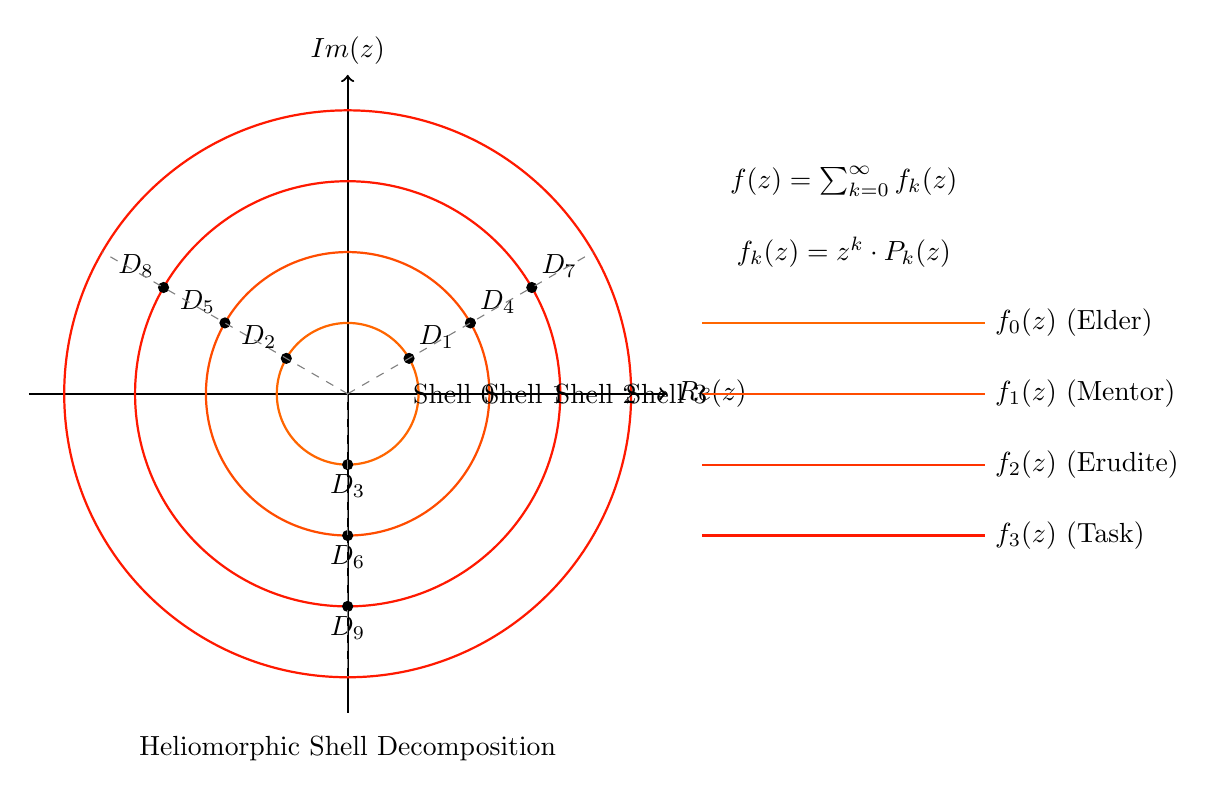
\begin{tikzpicture}[scale=0.9]
  % Define colors
  \colorlet{shell0}{orange!80!red}
  \colorlet{shell1}{orange!60!red}
  \colorlet{shell2}{orange!40!red}
  \colorlet{shell3}{orange!20!red}
  
  % Define the coordinate system
  \draw[->, thick] (-4.5,0) -- (4.5,0) node[right] {$\text{Re}(z)$};
  \draw[->, thick] (0,-4.5) -- (0,4.5) node[above] {$\text{Im}(z)$};
  
  % Draw concentric circles representing shells
  \draw[shell0, thick] (0,0) circle (1);
  \draw[shell1, thick] (0,0) circle (2);
  \draw[shell3, thick] (0,0) circle (3);
  \draw[shell3, thick] (0,0) circle (4);
  
  % Domain points at different positions
  \filldraw[black] (0.866,0.5) circle (2pt) node[above right] {$D_1$};
  \filldraw[black] (-0.866,0.5) circle (2pt) node[above left] {$D_2$};
  \filldraw[black] (0,-1) circle (2pt) node[below] {$D_3$};
  
  \filldraw[black] (1.732,1) circle (2pt) node[above right] {$D_4$};
  \filldraw[black] (-1.732,1) circle (2pt) node[above left] {$D_5$};
  \filldraw[black] (0,-2) circle (2pt) node[below] {$D_6$};
  
  \filldraw[black] (2.598,1.5) circle (2pt) node[above right] {$D_7$};
  \filldraw[black] (-2.598,1.5) circle (2pt) node[above left] {$D_8$};
  \filldraw[black] (0,-3) circle (2pt) node[below] {$D_9$};
  
  % Add radial lines to show domain alignments
  \draw[dashed, gray] (0,0) -- (3.464,2);
  \draw[dashed, gray] (0,0) -- (-3.464,2);
  \draw[dashed, gray] (0,0) -- (0,-4);
  
  % Representation of shell function decomposition
  \begin{scope}[shift={(7,0)}]
    % Shell decomposition equation
    \node at (0,3) {$f(z) = \sum_{k=0}^{\infty} f_k(z)$};
    \node at (0,2) {$f_k(z) = z^k \cdot P_k(z)$};
    
    % Function components for each shell
    \draw[shell0, thick] (-2,1) -- (2,1);
    \node[right] at (2,1) {$f_0(z)$ (Elder)};
    
    \draw[shell1, thick] (-2,0) -- (2,0);
    \node[right] at (2,0) {$f_1(z)$ (Mentor)};
    
    \draw[shell2, thick] (-2,-1) -- (2,-1);
    \node[right] at (2,-1) {$f_2(z)$ (Erudite)};
    
    \draw[shell3, thick] (-2,-2) -- (2,-2);
    \node[right] at (2,-2) {$f_3(z)$ (Task)};
  \end{scope}
  
  % Shell labels
  \node at (1.5,0) {Shell 0};
  \node at (2.5,0) {Shell 1};
  \node at (3.5,0) {Shell 2};
  \node at (4.5,0) {Shell 3};
  
  % Title
  \node at (0,-5) {Heliomorphic Shell Decomposition};
\end{tikzpicture}